\chapter{ISI}

\section{ORACLE APLICATION EXPRESS HR-1}
Oracle Apex adalah platform pengembangan kode rendah yang memungkinkan Anda membangun aplikasi perusahaan yang dapat diskalakan dan aman dengan fitur kelas dunia yang dapat digunakan di mana saja.Oracle apek juga merupakan lingkungan pengembangan perangkat lunak berbasis web yang berjalan pada database Oracle. Ini sepenuhnya didukung dan dilengkapi standar dengan semua edisi Oracle Database dan, dimulai dengan Oracle 11g, diinstal secara default sebagai bagian dari instalasi basis data inti. Data kode rendah pengembangan aplikasi, pertama adalah membuat database, membuat aplikasi, dan menyebarkan aplikasi yang sudah dibuat untuk dipublish. Dalam proses development ini adapula tahapan dalam start, antaralain new. New itu sendiri terdiri atas beberapa bagian antara lain markdown, model,SQL IDE,DML script, dan exel. Dalam proses tersebut maka akan dilakukan proses pengimputan data sql ke database. Selanjutnya akan di exiting menjadi aplikasi yang akan dibangun lalu aplikasi akan dites sebelum memasuki proses produksi pembuatan aplikasi. 
\begin{figure}[!htbp]
    \centering
    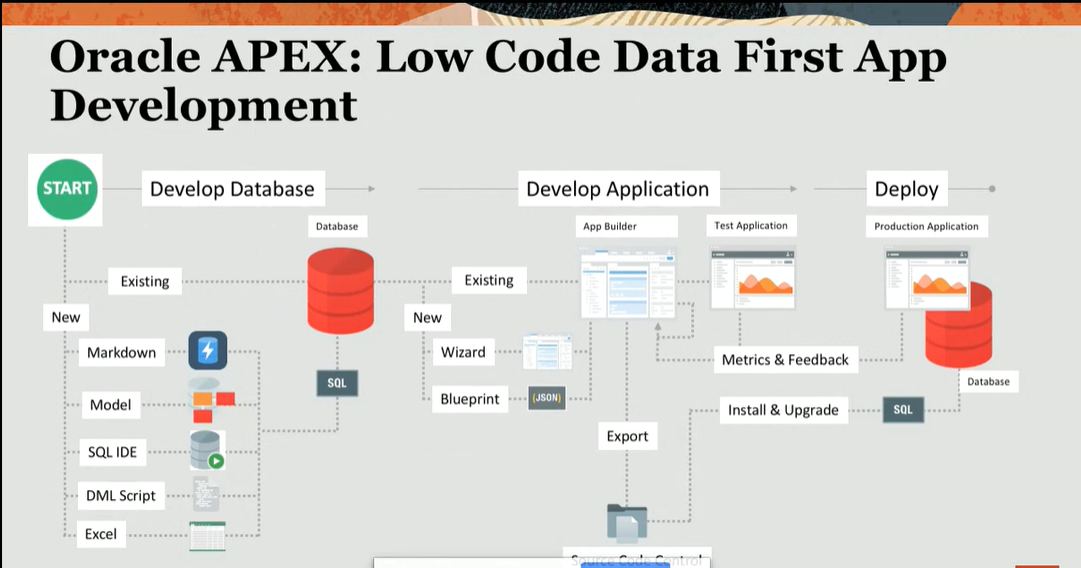
\includegraphics[scale=0.45]{section/hiya.PNG}
    \caption{proses pembuatan aplikasi pada oracle apex}
    \label{gambar 1}
\end{figure}



Mengelola data spreadsheet sangat menantang antaralain
  \begin{enumerate}
      \item Validasi data    -- manual dan rawan error
      \item Integritas data  -- tidak menjamin keakuratan data dalam lingkungan multiuser
      \item Keamanan data    -- penguncian sel tidak efektif
      \item Berbagi data     -- exel lamban dan sulit utuk dibagikan
  \end{enumerate}  
  
  Mengubah spreadsheet menjadi aplikasi web
  \begin{enumerate}
      \item Sign in apex.oracle.com
      \item Membuat workspace
      \item Buka app builder >create a new app>  drag dan drop file> pilih movie > next
      \item isi pada table nama, serta jenis huruf yang digunakan
      \item setelah itu create application lalu akan memasuki appreance yang dimana berisikan jenis- jenis tabel yang ada, pilih icon sesuai keinginan. pada feature centang semua kolom
      \item run aplikasi dengan memasukan kata sandi dan username
      
  \end{enumerate}
database centric framework pengembangan aplikasi web antara lain mengembangkan aplikasi web desktop dan seluler,memvisualisasikan dan memelihara data basis data,meningkatkan keterampilan sql dan kemampuan basis data. aplikasi  yang cocok dengan oracle apex antara lain aplikasi  yang kritis  memilikinmisi besar untuk ribuan pengguna, mengisi kekosongan dalam sistem perusahaan, proses bisnis kedaluwarsa steamline, modernisasi sistem lama, mengganti spreadsheet. 


Fitur dalam use case
\begin{enumerate}
    \item Melakukan drag dan letakkan file XLS, CSV, XML, atau JSON
    \item Membuat tabel dalam database otonom
    \item Mengunggah data ke tabel baru
    \item Membuat aplikasi berdasarkan tabel net
\end{enumerate}
 solusi dalam use case apex 
 \begin{enumerate}
     \item satu sumber jebakan
     \item mengirim URL bukan file
     \item scure, scalable, aplikasi multiuser
     \item melanjutkan dengan obrolan, kalender,validasi, dan lainnya
     
 \end{enumerate}
 
ORACLE APEX USE CASE
  \begin{figure}[!htbp]
    \centering
    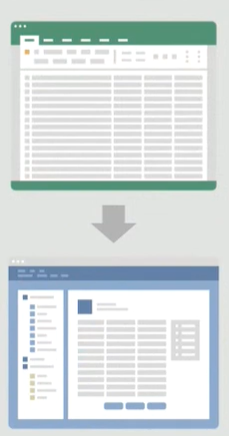
\includegraphics[scale=1]{section/1.PNG}
    \caption{penggantian pada lembar spreadsheet}
    \label{gambar 1}
\end{figure}
 
 Memodernisasi bentuk oracle
  \begin{figure}[!htbp]
    \centering
    
    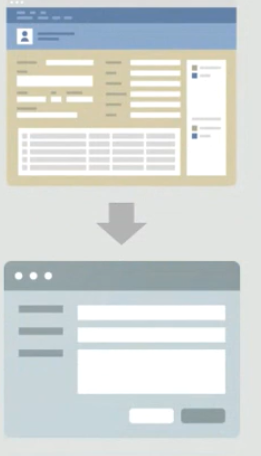
\includegraphics[scale=1]{section/2.PNG}
    \caption{memodernisasi bentuk oracle}
    \label{gambar 1}
\end{figure}
 